\chapter{Design Considerations for Implementing Halbach Arrays and High Temperature Superconductors for Contact-Free Flywheel Energy Storage Systems}
Christopher Mirabzadeh, Chris Birkinbine, Daniel Schneider, Joe Law, and Christine Berven

\begin{center}
Manuscript submitted on Sept. 2017 to \textit{IEEE Transactions on Applied Superconductivity} - Manuscript ID TAS-2017-0187
\end{center}

\section*{Abstract}
We have investigated the use of Halbach magnet arrays in combination with Type II High-Temperature Superconductors for use as a levitating thrust bearing for a fly-wheel energy storage system. Halbach arrays were selected because they have effectively one-sided flux and a greater flux gradient which would be expected to result in a greater levitation force and effective restoring force stiffness; each being beneficial in the design of such a system. To find the optimum orientation of the magnets for the arrays, we used Infolytica Magnet, a finite-element computation software package, to iterate over all permutations of magnet arrays costing of 3 and 5 magnets of single and double layers. The fields and levitation forces as well as the width of the magnet arrays relative to the width of the superconductor were analyzed.  Within our given design constraints, we found that, compared to a single magnet, a single-pole Halbach array was predicted to increase levitation force and stability, reduce stray fields, focus the flux, and increase the bearing stiffness.  We present our findings and suggest guidelines to increase levitation force of a superconducting magnetic bearing with qualifiers and rationale for optimizing such a system.  

\section{Introduction}
The NASA-sponsored, University of Idaho design team was tasked to design and build a solar energy storage system for reliable, efficient, and economical energy storage needs to power a lunar colony. This colony will consume an estimated 525 kW of power. The solar panels chosen as the main method of generating the required electrical energy require exposure to the Sun; however the moon cycles through 336 hours of sunlight and then 336 hours of darkness. During the hours of darkness no power will be generated from the solar panels. The UI design team designed a method to store energy for this period of darkness. 

Batteries, widely used for energy storage applications, were rejected because batteries are very inefficient at low temperatures found on the Moon. Most batteries deliver their power via a chemical reaction that produces electrical energy, when the temperature drops their chemical reaction slows and the battery cannot produce the same current it does at higher temperature leading to possible premature failure of the cell.  In addition, the cycle life, the number of complete charge - discharge cycles a battery can perform, is relatively short. 

As an alternative, chose a flywheel energy storage system for storing the required energy. Flywheels work by storing excess electrical energy as kinetic energy in a rotating system which may be stored for long periods of time or taken out as needed. Flywheels are environmentally clean, contain no hazardous materials, can efficiently store energy for long periods of time, have a long life expectancy (greater than 20 years), are ideally suited to multiple power applications, can handle rapid discharge rates without degradation, and are easier to maintain versus other options. Flywheels are typically constructed of steel and rotate on conventional contact bearings; however, contact bearings incur energy losses from friction.  The UI design team chose to use magnetic levitation via high temperature superconducting (HTS) magnetic bearings because it has been suggested as a method to remove those energy losses \cite{xia, miyazakim, fang, cansiz, strasik, sung, sotelo2, nagashima, birkner, werfel, coombs002, ma, mulcahy1,choi}. 

High temperature superconducting magnetic bearings (SMB) have challenges of their own.  First, it is very difficult to control free bearings as they are analogous to a spinning top with no fixed point and multiple degrees of freedom.  Second, an SMB may have its natural resonant frequencies stabilized with the aid of an active magnetic bearing or by the mechanism of flux trapping.  Additionally a superconducting magnetic bearing will have a decrease in levitation force over time due to flux creep \cite{miyazakim, suzuki, postrekhin}.  There are also rotational energy losses that must be considered because SMB's are not completely friction free.  There are at least three sources of energy loss\cite{xia, sotelo2}; (a) windage due to motion of the rotor in a fluid, (b) thermal losses from radiation, convection and conduction and (c) hysteresis losses due to inhomogeneities in the magnetic field.

\section{Methods}
The UI Design team chose to use superconductor bearings instead of traditional bearings because they are materials that conduct electricity with zero resistance and completely expel magnetic fields when cooled below a characteristic critical temperature. This makes HTS attractive since these temperatures are easily accessible using Liquid Nitrogen. All superconductors expel magnetic fields when cooled below a characteristic critical temperature. The critical temperature of type I superconductors require temperatures well below 77K, whereas the critical temperature of type II high temperature superconductors is well greater than 77K. The difference between a Type I and Type II superconductor, besides the critical temperature, is that Type II superconductors have two critical fields.  Between the critical fields lies a mixed-state where the superconductor traps magnetic flux and hence the Meissner Effect is not complete.  Thus, high temperature superconductors cooled with Liquid Nitrogen can be used to stably levitate permanent magnets. For a review of superconductors and their properties see Tinkham \cite{tinkham}.

 A number of authors have already explored superconducting magnetic bearings and flywheel energy systems \cite{xia, miyazakim, cansiz, sung, nagashima, werfel, coombs002, ma, mulcahy1, turner, ikedia}.  In addition, Halbach arrays have been optimized for use by Maglev levitation vehicles \cite{Jing, deng, zhang, del2, liu, deng2} and in motor designs \cite{turner, soltner, robertson, wang}.  In this section we mean to present our procedure for selecting the appropriate magnetic array for all of our requirements and constraints.  We then present several different array configurations based on these preliminary findings based on Finite Element Analysis (FEA) methods and finally experimental methods to confirm and rationalize the final recommendations.

The levitation force must be large enough to support the rotor mass we must consider practical constraints such as size and spatial volume.  Selecting neodymium permanent magnets were chosen because of their high residual magnetization and because  small volume permanent magnets will always outperform iron core electromagnets in a small dimension space\cite{hawkins}. Selecting these magnets enabled us to increase the relative force per volume ratio which reduces the number of magnets needed for levitation.  For the initial phase of the project we considered using alternating magnetic rings such as those used in similar projects \cite{strasik, sotelo1}.  Calculations proved such a magnet to have sufficient force to levitate our rotor design; however, the design and manufacture was deemed cost prohibitive.  Instead, we researched smaller, “off the shelf”, magnets.  We further discovered that stray flux could be decreased and magnetic stiffness increased if we formed the magnets into radial Halbach arrays.  

A Halbach array, also called a “flux sheet” by Mallinson \cite{mallinson}, is a simple arrangement of permanent magnets that effectively doubles the field on one side, the active face, and reduces stray fields on the opposite side, the “inactive face”.  See Fig. \ref{fig_halbach} for a simple arrangement.  Halbach arrays are common in brushless motors \cite{Hull1, zhu} and are seeing an increased use in magnetic levitation rail trains \cite{ham, Jing, post}, flywheel energy systems \cite{sotelo2, turner}, and Nuclear Magnetic Resonance (NMR) \cite{raich, soltner}. Also, since the field is reduced on the inactive face, we expect use of Halbach arrays to be beneficial in reducing the magnetic interference between the rotor and stator.  

One of our goals was to produce as much magnetic force as possible per unit area.  There is computational and experimental evidence that the Halbach array superconductor system is superior to a permanent magnet and superconductor system \cite{sotelo2, Hull1, Jing, turner, del1, deng, zhang, del2, liu, deng2}.  A levitating halbach system shows increased levitation force, increased stiffness and enhanced stability.  On average the levitation force between a halbach array and superconductor has been shown to be 2.3 times that of a single permanent magnet and superconductor \cite{Jing}.  FEA shows that the Halbach array configuration is capable of obtaining the same magnetic force for larger gaps between rotor and stator as compared to using iron shim flux shapers \cite{sotelo2}.

Maximum levitation force is attainable by first cooling the superconductor far from any magnetic field \cite{ma, Hull1999, del1, zeisberger2}.  This is called zero-field-cooling (ZFC). Flux Creep causes time relaxation in the levitation force.  This problem is resolved by preloading the SMB before initial rotation \cite{miyazakim, suzuki, postrekhin, ma}.

Cooling the superconductor near a magnet source is called field cooling (FC) and although this configuration has been shown to  reduce the levitation force, it improves the lateral stability due to pinning \cite{ma, Hull1999, del1}.
A field cooled system is less susceptible to flux creep because the HTS resists any changes in the external field \cite{xia}.

Werfel et al. have emphasized design rules for HTS bearings \cite{werfel}.  
\begin{quote} 
Acheiving high bearing stiffness requires a multipole arrangement of the magnets.  If the air gap is larger than 4-5 mm, due to magnet bandage or thermal isolation, a reduced number or even a single magnet pole may give better force-density values. 
\end{quote}

It has been recognized that edge effects between superconductors and magnets directly affect the levitation force \cite{ma, Jing}.  Therefore the width ratio, fixed width halbach array versus variable width HTS, and field cooling height must be considered a characteristic of the overall system specifications.

Del-Valle \cite{del1} have shown that as the ratio of the width of the superconductor to the magnet array increases so does the stabilizing force; however, when the width is large enough as to completely cover the total width of the magnet array simpler arrangements may be the better configuration due to the magnetic field profiles.  Furthermore, they suggest having a height of the permanent magnet larger than that of the superconductor.

In an evacuated system we may ignore windage and thermal losses except by radiation; however, magnetic hysteresis loss has been shown to depend on the amplitude of changes in the B-field on the surface of the superconductor \cite{coombs003}.  This implies that any changes in frequency, which creates a change in the B-field at the surface of the superconductor, will create rotational losses.  These hysteresis losses are analogous to frictional drag \cite{ma}\cite{turner}.  Inhomogeneities in the magnetic field of the permanent magnets lead to time-varying magnetic fields on the surface of the superconductor, i.e. a conductor moving through a non-uniform magnetic field induces eddy currents and thus contributes to energy losses.

Spin up and spin down tests have shown rotational losses to be a function of temperature and height between a rotor magnet and superconductor \cite{cansiz,  werfel}.  It was shown that the smaller gap distance, 4mm compared to 5mm, increases hysteresis losses due to higher field variations experienced by the superconductor.  The observed decay rate in the spin down test has been used to approximate a relative coefficient of friction with a range in magnitude from $10^{-5}$ to $10^{-8}$ \cite{cansiz}

\subsection{Computational}
Based on the selection criteria outlined above we considered arrays made of 3 and 5 permanent magnets to produce a target levitation height greater than 5 mm. Three magnets can be used to create a single pole and five to create a double pole.  In order to determine the greatest levitation force per unit area, different magnet orientations were simulated using finite element analysis with the finite element package Infolytica - MagNet, version 7 \footnote{http://www.infolytica.com/}.  Only the levitation force was considered.  ZFC and the Meissner effect are assumed.  Idealized materials restrict our simplified model to closer resemble Type I superconductors.

Orientations considered were all possible permutations of 3 and 5 magnet arrays such as those pictured in Table \ref{tab_nonlin}.  Other configurations included separating the magnets with iron shims, and 1 layer  versus 2 layers as 2 layers will have a height larger than that of the superconductor as suggested by Del-Valle \cite{del1}.

\begin{table}[ht]
\caption{Proposed magnet arrays} % title of Table
\centering % used for centering table
\begin{tabular}{cc} % centered columns
\hline % inserts single horizontal line
\
\\
$90^\circ$ Roll Angle & $\uparrow \rightarrow \downarrow \leftarrow ...$ \\ % inserting body of the table
\\
Alternating Iron(I) Shims & \framebox{I} \framebox{$\rightarrow$} \framebox{I} \framebox{$\uparrow$} ... \\
\\
Iron Shims Outside the array & \framebox{I}  \framebox{$\rightarrow$} \framebox{$\uparrow$} \framebox{$\leftarrow$}  \framebox{I}\\
\\
1 Layer & \framebox{$\rightarrow$} \framebox{$\uparrow$} \framebox{$\leftarrow$}\\ [1ex] % [1ex] adds vertical space
\\
2 Layers &  \framebox{$\rightarrow$} \framebox{$\uparrow$} \framebox{$\leftarrow$} \\
& \framebox{$\rightarrow$} \framebox{$\uparrow$} \framebox{$\leftarrow$} \\
\\
\\
\hline
\end{tabular}
\label{tab_nonlin} % is used to refer this table in the text
\end{table}

Fully 3D periodic boundary conditions were possible but not necessary to find the desired results.  Slab boundary conditions are useful for simulating a part of a system of planar surfaces (e.g. x and y) with periodic boundaries while leaving the third (z) direction remaining vacuum to infinity.  The model is shown in Fig. \ref{fig_2DModel}.  As shown, the model is 2D which assumes an infinite z dimension. Unless otherwise stated, the HTS was 35 mm wide and 6.35 mm tall.  The magnets were 6.35 mm cubes in order to represent easily obtainable "off-the shelf" magnets.  This limited the angle between any adjacent pole to multiples of $90^{\circ} $.

The 2D simulation is limited, however, Type II superconductors can be modeled with a magnetic permeability less than that of air.  Passive magnetic levitation needs a relative permeability of less than 1.  The relative permeability for the material HTS was set to $10^{-5}$.  This simulates the diamagnetic property of superconductors to oppose an externally applied magnetic field.  The boundary conditions must also be set such that there is zero normal magnetic flux for field cooling.  This allows flux penetration when using a non-linear solver based on the critical state model.  For ZFC the boundary condition is zero vector potential which allows flux to be expelled from the superconductor.

Within the simulation we performed three experiments: 1) Force as a function of height where the HTS positioned 56 mm above each array and was lowered by 1 mm increments.  2) Force as a function of HTS width.  3) Force as a function of array stacks.

\subsection{Experimental}

We purchased 23 seeded, melt growth, superconducting, single domain, YBaCuO (YBCO)  HTS levitation disks for our experiments and flywheel construction from Can Superconductors \footnote{http://www.can-superconductors.com/}.  The wedge shape of the YBCO (Fig. \ref{fig_HTS_Samples}) was pre-selected in order to create a ring when all of the superconductors were fitted together in the final flywheel construction. The HTS were cataloged and referenced as SC0XX, where XX was a number from 01 to 23.  There were no visual defects and all HTS arrived with a clear protective coating. The interaction force between the Halbach array and HTS was measured using the force jig shown in Fig. \ref{fig_forcejig}.  The force jig was constructed of brass in order to limit magnetic interactions.  The force jig consisted of an electro-balance (TREE Model:HRB20001) with a 0.1 g resolution and a 20 kg capacity to quantify the forces.  The interchangeable magnet block assembly, either composed of 8 double layered or single layered periodic arrays in the orientation  $\rightarrow \uparrow \leftarrow$, was placed on the modular tray. The radius of curvature for the block assembly was 3.3375" to the center of the magnets same as the final ring assembly.  We used N-52, 6.35 mm cube magnets purchased from K \& J Magnetics.  The arrays were glued together using a metal compression jig, Gorilla glue, and High-Density Polyethylene (HDPE) to ensure the magnets did not glue to the metal jig. The magnetic field at the surface of the magnets and center of the arrays was measured using a Lakeshore 421 Gaussmeter.  The averages are shown in Table \ref{tab_gauss}.

\begin{table}[htbp]
  \centering
  \caption{Average magnetic field measured with a Lakeshore 421 Gaussmeter and attached Hall probe.  The measurements were taken at the center surface of each configuration shown. }
    \begin{tabular}{rrr}
    \hline
                            & 1 Layer                      & 2 Layers\\
    \hline
   1 Cube Magnet	&	0.555T	&	0.626T\\
   3 Magnets $\uparrow\uparrow\uparrow$		 & 0.581T & 0.644T \\
   3 Magnets $\rightarrow\uparrow\leftarrow$ & 0.750T & 0.834T \\
    \hline
    \end{tabular}%
  \label{tab_gauss}%
\end{table}%

The HTS sample was placed in a plastic cup and secured by a pressure rod.  The magnet block was centered on the modular tray below the cup holder of the force jig. For ZFC, the cup with superconductor was cooled "infinitely" far from the force jig.  As Liquid Nitrogen has a tendency to boil as it comes into contact with warmer solids we allowed the boiling to settle after filling the cup and superconductor and an additional minute passed before placing the cup into the force jig.  Liquid nitrogen was replaced as needed.  The apparatus started at a height of 56 mm and was lowered in 1.25 mm (0.05 in.) increments.  At each increment the scale was read and the force recorded. The HTS were then characterized by their individual levitation force and fit to an exponential function as shown in Table \ref{tab_expfitparm}. 

\section{Results}
For the computational results, flux and force profiles were generated for each permutation of single and double layered magnets using the FEA package. Because we were constrained to off-the-shelf cube magnets, all roll angles between any two consecutive magnets must be  $90^{\circ}$, where we defined the roll angle as the angular difference between two consecutive dipoles. We generated 2176 permutations in all. In order to reduce the number of profiles to be considered we constrained our selection with a set of rules:

\begin{enumerate}
\item Stray magnetic fields may interact with and cause energy losses between the stationary stator and rotating rotor in the air gap between the two.  In order to reduce stray fields and maintain one-sided flux we only considered periodic arrays similar to Halbach arrays.  This means that for any three magnets $A, B, C, A \neq B \neq C$.
\item There is symmetry through the permutations i.e. the orientation $\uparrow \uparrow \leftarrow$ only appeared once but had the same force and flux profile as $\downarrow \downarrow \rightarrow$.  This can be seen in Table \ref{tab_greatforce}. Therefore, profiles with degenerate solutions were unnecessary to consider and discarded.
\item Through consideration of project constraints it was determined that 3 magnets in two stacks would be sufficient to supply the needed force. 
\item It was decided that a potential well of magnetic flux would add some stability despite the fact that we are using ZFC.  Therefore, profiles without the required flux geometry were removed. 
\end{enumerate}

\begin{table}[htbp]
  \centering
  \caption{The data shown here is ordered to show orientations with greatest force profile in the range of interest.  The orientation is that of the magnetic field inside the magnet where U= up, R=right, L=left, and D=down.}
    \begin{tabular}{rrr}
    \hline
    Profile                        & Force(N)                       & Orientation \\
    \hline
    3                              & 4.51                       & UUL \\
    62                             & 4.51                       & DDR \\
    17                             & 4.50                       & RUU \\
    48                             & 4.50                       & LDD \\
    11                             & 4.41                       & ULL \\
    54                             & 4.41                       & DRR \\
    21                             & 4.40                       & RRU \\
    44                             & 4.40                       & LLD \\
    19                             & 4.18                     & RUL \\
    46                             & 4.18                       & LDR \\
    12                             & 4.13                       & ULD \\
    53                             & 4.13                       & DRU \\
    1                              & 3.33                       & UUU \\
    64                             & 3.33                       & DDD \\
    43                             & 3.01                       & LLL \\
    22                             & 3.01                       & RRR \\
    \hline
    \end{tabular}%
  \label{tab_greatforce}%
\end{table}%

The configurations that best met the above criteria were profiles 12 and 19, shown in Figures \ref{fig_fluxprofile_12} and \ref{fig_fluxprofile_19} respectively. Profile 12 was rejected due to smaller force profile and lacked the desired flux geometry.  Thus, two stacks of 3 magnets with profile 19, Fig. \ref{fig_fluxprofile_19}, were found to be the minimum fit for all arguments of space, volume, force and stability.  The force curve for profile 19 with one and two stacks of magnet arrays are shown in Fig. \ref{fig_force19_one} and Fig. \ref{fig_force19_two} respectively.

Experiments using profile 19 were conducted using the above described force jig.  The results for one and two stacks of magnet arrays are shown in Fig. \ref{fig_force22_one} and Fig. \ref{fig_force22_two} respectively.

\section{Discussion}
An analytical model for forces between superconductors and Halbach arrays in the ZFC orientation can be achieved using the method of images, a qualitative approximation for determining the force between a superconductor and permanent magnet system \cite{perez, yang, kordyuk, saslow, Hull1999, tsuch2}. However, the image method is unable to account for edge effects and irreversible magnetization due to vertical displacements \cite{Hull1999}.  When flux penetration occurs, Bean's critical state model will be needed in order to work out the resistance to motion in all directions \cite{ma, tsuch2, ruiz, bean2, davis, del1}.  In order to create a model for the interaction between a Halbach array and HTS we also needed to consider the theoretical model for the "flux sheet" which deals with the phenomena of one-sided flux as derived by Mallinson \cite{mallinson}.  We could also consider a more rigorous interpretation of the method of images such as in \cite{perez}. 

Intuitively, we expected decreasing values in the force as the distance between the HTS and Halbach arrays increased but at this point we are not speculating as to why and reserve a deeper analysis for future works.  A semi-log plot is most useful when one suspects an exponential fit of the form:

\begin{equation}
F=F_0 e^{(\frac{-x}{x_0})}.
\end{equation}

Thus the experimental data was fitted to a semi-log plot as shown in Fig. \ref{fig_force22_two}.  The resulting graph is a near straight line which reinforced our suspicions.   The data was fitted and the fitting parameters are shown in Table \ref{tab_expfitparm}.

\begin{table}[!t]
  \centering
  \caption{Fitting parameters for experimental force data between the HTS and 8 double arrays of profile 19 arranged in a semi-circle to represent a piece of the flywheel to be constructed. The data starts at a height of 15 mm which is the maximum range of interest.}
    \begin{tabular}{cccc}
    \hline
    & \textbf{$F_0(N)$} & \textbf{$x_0(mm)$} & \textbf{$R^2$} \\
    \hline
    \textbf{SC001}& 18.44& 4.78& 0.9999 \\
    \textbf{SC002}& 19.51& 4.69 & 0.9998 \\
    \textbf{SC003}& 20.58& 4.67 & 0.9997 \\
    \textbf{SC004}& 21.01& 4.59 & 0.9999 \\
    \textbf{SC005}& 20.04& 4.67 & 0.9997 \\
    \textbf{SC006}& 18.67& 4.90 & 0.9995 \\
    \textbf{SC007}& 18.45& 4.86 & 0.9997 \\
    \textbf{SC008}& 18.75& 4.73 & 0.9999 \\
    \textbf{SC009}& 20.1 & 4.80 & 0.9997 \\
    \textbf{SC010}& 19.55& 4.78 & 0.9994 \\
    \textbf{SCO11}& 20.65& 4.75 & 0.9996 \\
    \textbf{SC012}& 19.61& 4.82 & 0.9997 \\
    \textbf{SC013}& 19.53& 4.82 & 0.9997 \\
    \textbf{SC014}& 19.82& 4.61 & 0.9997 \\
    \textbf{SC015}& 20.69& 4.65 & 0.9997 \\
    \textbf{SC016}& 19.01& 4.60 & 0.9999 \\
    \textbf{SC017}& 20.53& 4.59 & 0.9998 \\
    \textbf{SC018}& 19.87& 4.55 & 0.9999 \\
    \textbf{SC019}& 18.55& 4.74 & 0.9997 \\
    \textbf{SC020}& 18.39& 4.78 & 0.9996 \\
    \textbf{SC021}& 20.54& 4.63 & 0.9998 \\
    \textbf{SC022}& 18.06& 4.78 & 0.9999 \\
    \textbf{SC023}& 20.41& 4.73 & 0.9996 \\
    \textbf{ Mean}&	19.60&4.72	&0.9997\\
	\textbf{Std. Dev.}	&0.88	&0.10	&0.0001\\
    \hline
    \end{tabular}%
  \label{tab_expfitparm}%
\end{table}%

All of the simulations were solved using the available Infolytica Magnet Static 2D solver. As a 2D approximation neglects fringing and leakage in the material, fringing and leakage in the material and rotational geometry are better simulated in 3D; however, our FEA simulation was strictly used as a means for initial decision making, therefore 2D approximations were deemed appropriate.   Accuracy was further improved by steadily increasing the polynomial order and decreasing the element size of the mesh by automated adaption. 

The simplified 2D model we used was idealistic and closer to the characteristics of Type I Superconductors.  The limitations of the model were: idealized materials, assumed Meissner state, ZFC, only the levitation force was considered, only static solutions, which implies no induced currents from moving magnetic fields therefore AC losses from pinning effects and eddy currents were also ignored. A nonlinear solver was beyond the scope of our initial considerations and not necessary with the assumption of ZFC.  A nonlinear solver was deemed appropriate for the inclusion of pinning and flux penetration in our future works.

Other, stronger configurations are possible, however, not within our given constraints. As shown in Table \ref{table_stacks}, the simulation data predicted that adding additional stacks of the same orientation have the effect of increasing the force but any improvement falls off quickly as the number of stacks increases and is not as great after the third stack. Data using alternating iron shims was excluded due to the lack of required minimum force.  Although iron shims are useful for shaping flux lines the absorption of the field lines into the iron reduces the number of field lines seen by the superconductor, therefore reducing the total force on the superconductor.  Halbach arrays also offer the required flux shapes that we needed.  Different geometries should be considered dependent upon different configuration.

\begin{table}[!t]
\caption{Simulation data of the force between HTS and different layered stacks of array 19 at a height of 6.35mm using FEA}
\label{table_stacks}
\centering
\begin{tabular}{cc}
\hline
Number of layers & Force(N) \\
\hline
One & 4.18\\
Two & 7.93\\
Three & 10.19\\
Four & 11.59\\
Five & 12.49\\
Six & 13.10\\
\hline
\end{tabular}
\end{table}

In comparing the force from array 1 ($\uparrow \uparrow \uparrow $), where all of the magnets are in the same direction, to the force of a dipole magnet of similar volume consider Table \ref{tab_greatforce}.  From the table we may compare profile 1, Fig \ref{fig_fluxprofile_1},  with the configuration $\uparrow \uparrow \uparrow$ to any of the periodic arrays and see that the single direction magnet arrays have less force than any given periodic array.  The force from profile 1 is 1.3 times less than our chosen profile, 19.  

SMB's are typically associated with low bearing stiffness since they can not sustain a large fluctuation in load. Bearing stiffness is defined by how the airgap between the rotor and stator varies under load.  The force between the two opposing surfaces is greatly dependent on the flux density gradient of the airgap. Thus the stiffness of a magnetic bearing would vary as the magnetic field varies. The periodic array focuses the flux to one side of the array creating a more sinusoidal waveform and shortened flux lines due to the interaction between the poles of the individual permanent magnets.  This leads to an increase in the flux density gradient in the airgap.  Further, when compressed, the increased magnetic flux of periodic arrays tend to smooth out the variance in the magnetic field. By increasing flux density and decreasing field variance the periodic arrays have the effect of increasing bearing stiffness. Figures \ref{fig_BFieldSnLs} and \ref{fig_BFiledDbLs} show the higher magnetic field strength of array 19 compared to a single cube magnet and array 1 which represents a rectangular magnet of the same physical volume of array 19.

The original reasoning for increasing the number of layers of magnets was suggested by Del-Valle \cite{del1} in order to have the height of the permanent magnet greater than that of the superconductor and was expected to increase the magnetic field strength.  Our simulations also predicted that increasing the number of array layers would significantly increase the force on the superconductor but our experiments did not mirror the same result.  What we found in comparing the data, Fig. \ref{fig_1layervs2}, is that there was a greater force using multiple layers of magnet arrays at distances greater than 15 to 20 mm.  However, at that point the increase in force fell off to 1.5 times greater and down to near equal force at the heights we are interested in, 5 to 7 mm.  An increase in magnetic field increased the number of flux lines seen by the superconductor.  More flux lines equals more force per unit area, or more magnetic pressure; however, as a ZFC type II superconductor got closer to a magnetic field, flux lines were penetrating and experiencing creep from atomic defects.  Thus intrinsic disorder was of crucial importance in understanding superconducting states.  The decreased force and the slow response to an applied force, which we've seen in the experiments, was likely due to the intrinsic properties of Type II Superconductors. Therefore we saw that more stacks were not advantageous at heights of 5-7 mm. The experiments showed that one stack had a similar force profile as two stacks at short distances.

Given the apparent exponential form for the force as a function of height, we predicted that the effective differential static spring rate would be equal to the negative of the force at a given height divided by the decay length in the argument of the exponent. As could be expected, with a single layer of magnets where the magnetic flux density gradient is larger, the decay length would be shorter which would result in a larger effective spring rate. This can be seen to be consistent with the experimental data, Fig \ref{fig_1layervs2}, in the slopes of the $F(x$) curves at about x = 6mm where the levitation force for both the single and double layer configurations have the same value but the slope is steeper for the single layer case.

When considering stability, our model (and Del-Valle's) showed that the superconductor should be wide enough to completely cover the width of the magnets, Fig \ref{fig_ForceWidthArr19}.  Although the levitation force decreased when the width ratio was above 1 to 1, for the chosen configuration we saw no significant decrease once the width ratio is 1.3 times wider than the magnet array.  Although there was a small decrease in the levitation force, we expected that an increased width ratio maximized the surface area of the magnetic flux seen by the superconductor and therefore maximized the compression area and increased the horizontal stability.  

\section{Conclusion}

The results of a two-dimensional finite element analysis using idealized material properties was assessed and compared to the measured repulsive force between arrays of magnets and high temperature superconductors. The use of Halbach arrays with nearly one-sided flux profiles were investigated with the expectation that this type of flux profile would increase the repulsive force between the magnets and superconductor and increase the effective static spring-rate of the interaction. 

Evaluating the effect of adding additional layers of magnets was also investigated, both experimentally and through simulations. It was expected that the greater flux density would result in both a greater force for all heights and also a greater effective static spring rate. Although the addition of a second layer of magnets did increase the force for most of the height range of interest, an additional layer of magnets did not result in a larger levitation force for the smaller heights and also decreased the differential static spring rate over the whole range of interest. The difference between the measured and simulated forces was possibly due to complications associated with the physics of flux penetration into the superconductor that the model used here was not intended to simulate; however, for initial characterization, the simplified model was found to be sufficient to aid in evaluating permanent magnet array configurations with much smaller investment in software.

A 2D Finite Element Analysis is limited in its ability to predict the interactions between magnets and High Temperature Superconductors.  The simulation data is only appropriate for initial guess work and tells us very little of the underlying physics.  In order to more accurately account for flux penetration and leakage, a 3-dimensional, non-linear solver is required.  On average the levitation force between a Halbach array and superconductor has been shown to be as much as 2.3 times that of a permanent magnet and superconductor\cite{Jing}.  This is due to the one-sided flux created by the rotation angle of the magnetic dipoles.  One-sided flux increases flux density which increases bearing stiffness.  Periodic magnet configurations with increased field gradients are expected to provide higher bearing stiffness.  Therefore, the Halbach array focuses flux, allows for flux control, and increases levitation stiffness.  Simple arrays of 3 magnets are better for maximizing force considerations since in a 3 magnet array there is effectively only one pole, therefore the flux interacts with other poles further away.  To increase the force even more, one may stack the arrays; however, additional layers may decrease the overall bearing stiffness due to flux penetration in type II superconductors and further shortening of flux lines due to pole interactions.  Also, more than two stacks show less of an increase in overall levitation force and considerations should be made for the usable volume space. When considering more stable configurations, width ratios greater than 1.3:1 for superconductor to magnet array shows no considerable reduction in levitation force. The decrease in levitation force due to time dilation caused by flux creep is expected to be minimized by either pre-loading the flywheel before initial rotation or by field cooling.  Pre-loading and field-cooling allows the HTS to better resist any changes in the external magnetic field.


% use section* for acknowledgement
\section*{Acknowledgment}
We would like to thank Infolytica Corporation for the use of their Finite Element Package, MagNet, and Dr. Gilles Fillion for his instructive and timely correspondence.  Funding for this research was provided by The NASA Ralph Steckler Space Grant.

\pagebreak 

\begin{figure}[htbp]
\centering
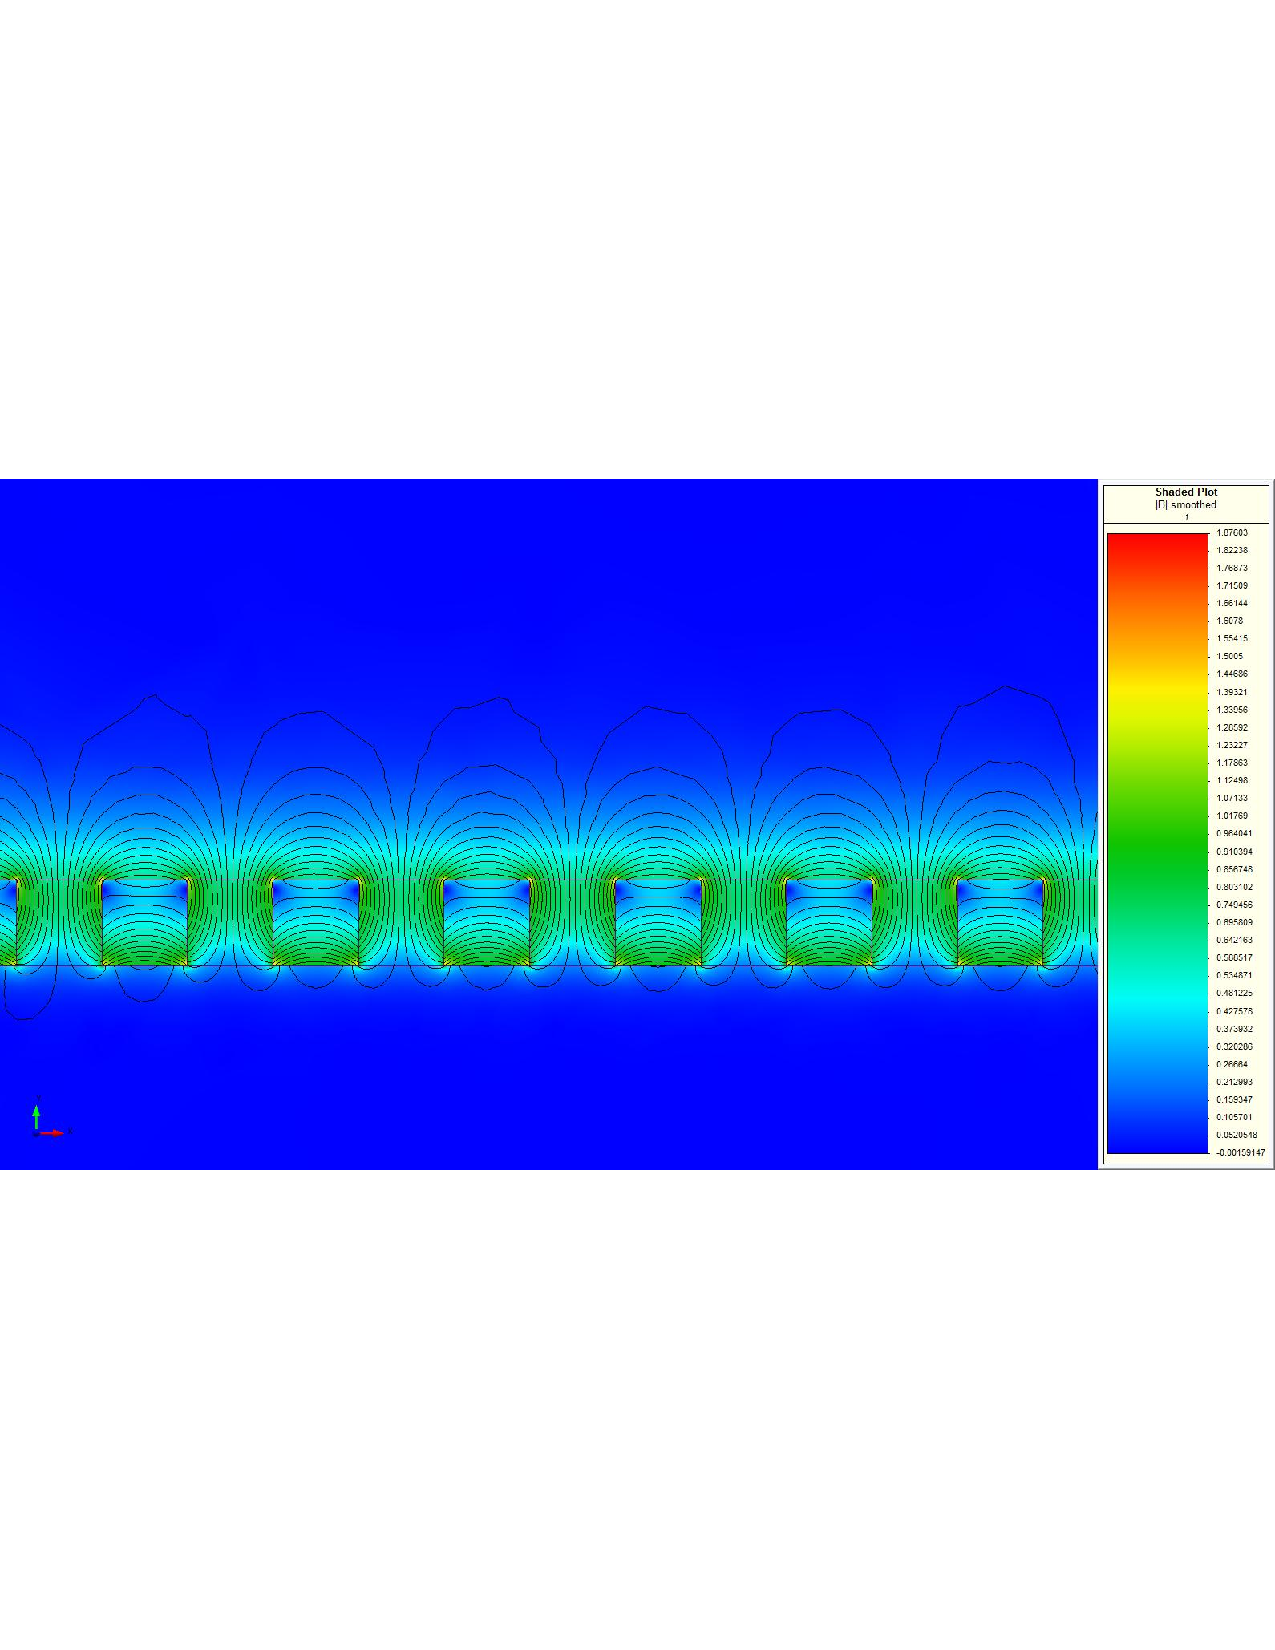
\includegraphics[scale=0.65, clip=true, trim=5cm 10cm 5cm 10cm]{typical_halbach_array.pdf}
\caption{A simulation of an infinitely repeating Halbach array.  The black lines are the flux lines and the gradient colors represent the magnetic field gradient.}
\label{fig_halbach}
\end{figure}

\begin{figure}[htbp]
\centering
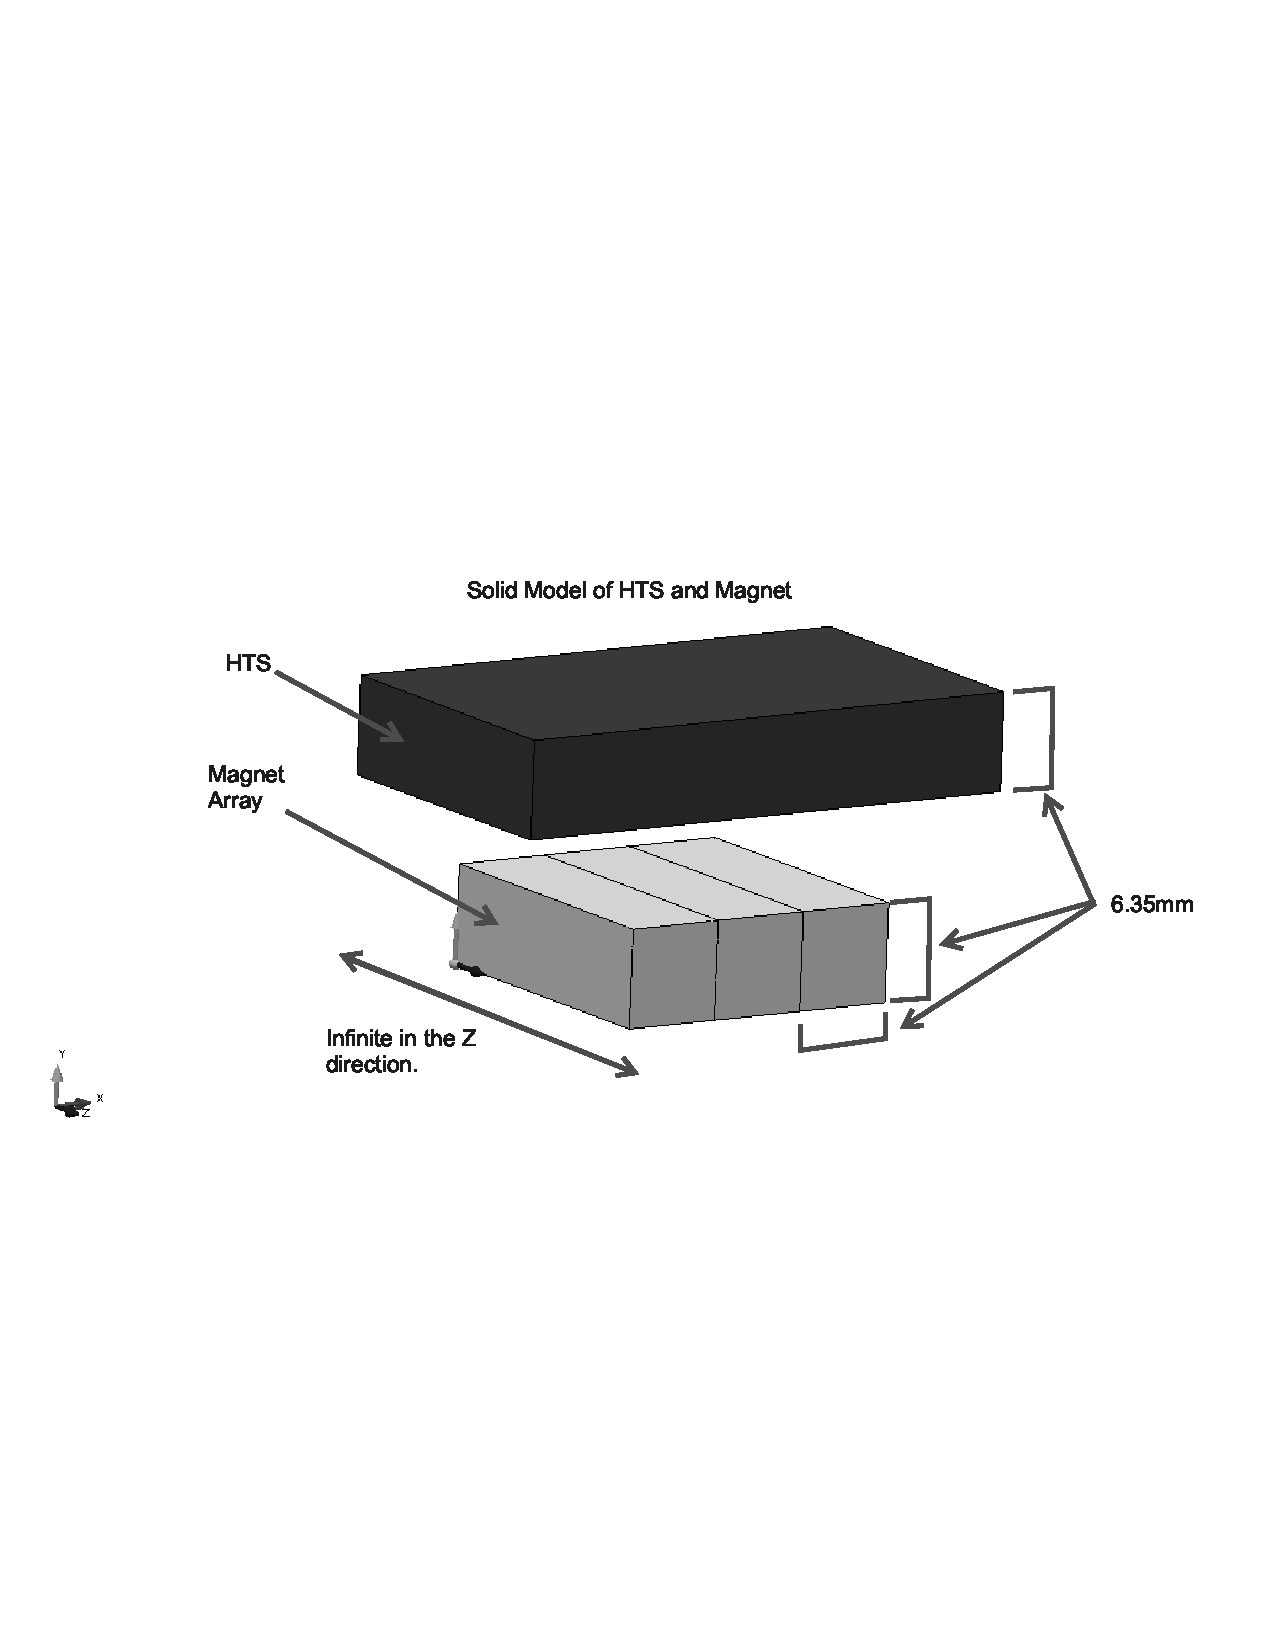
\includegraphics[scale=0.45, clip=true, trim=3cm 8cm 0cm 8cm]{2DModelHTSArray.pdf}
\caption{Two dimensional solid model generated by Infolytica Magnet 7 representing slab boundary conditions with an air box 10 times larger than the unit cell shown.  The z direction is considered infinite.}
\label{fig_2DModel}
\end{figure}

\begin{figure}[htbp]
\centering
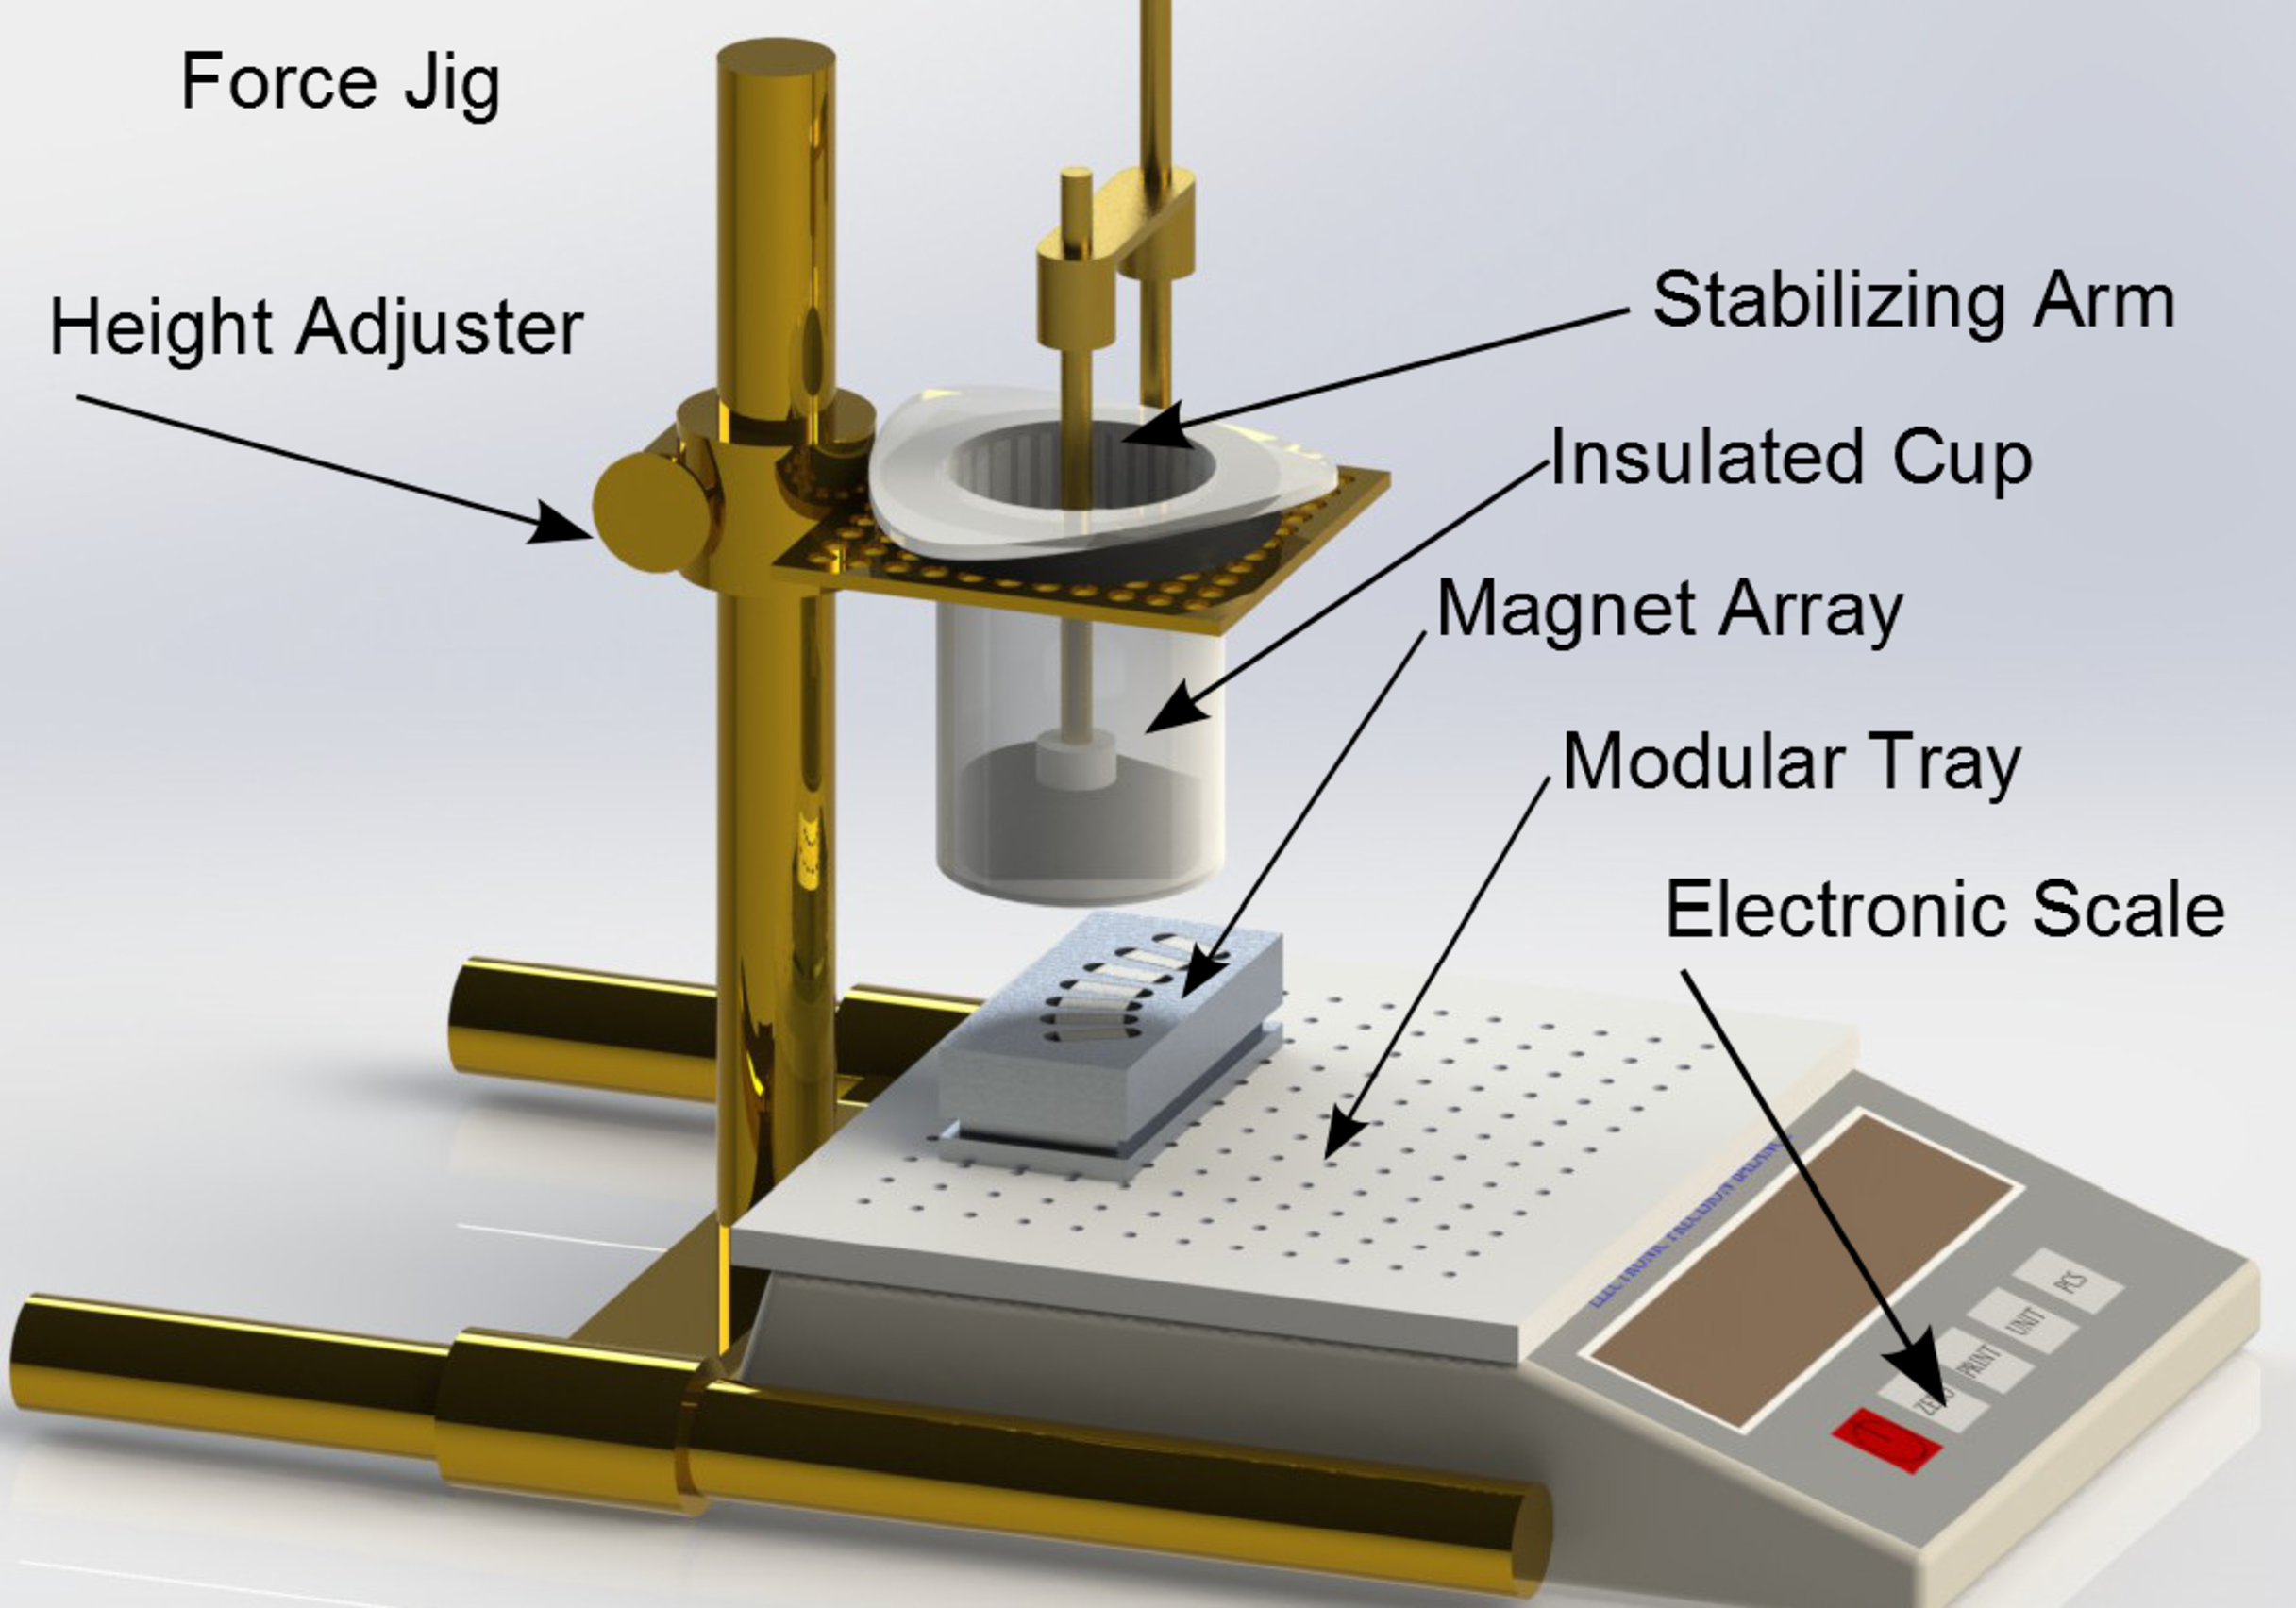
\includegraphics[scale=0.2]{forcejig.pdf}
\caption{Solid model of the Force Jig used to measure the interaction force between superconductors and magnet arrays.  The jig was constructed of brass to maintain low magnetic interference.  The tray of the balance was replaced with a Polythylene modular tray constructed to secure magnet arrays in different orientations as needed.}
\label{fig_forcejig}
\end{figure}

\begin{figure}[htbp]
\centering
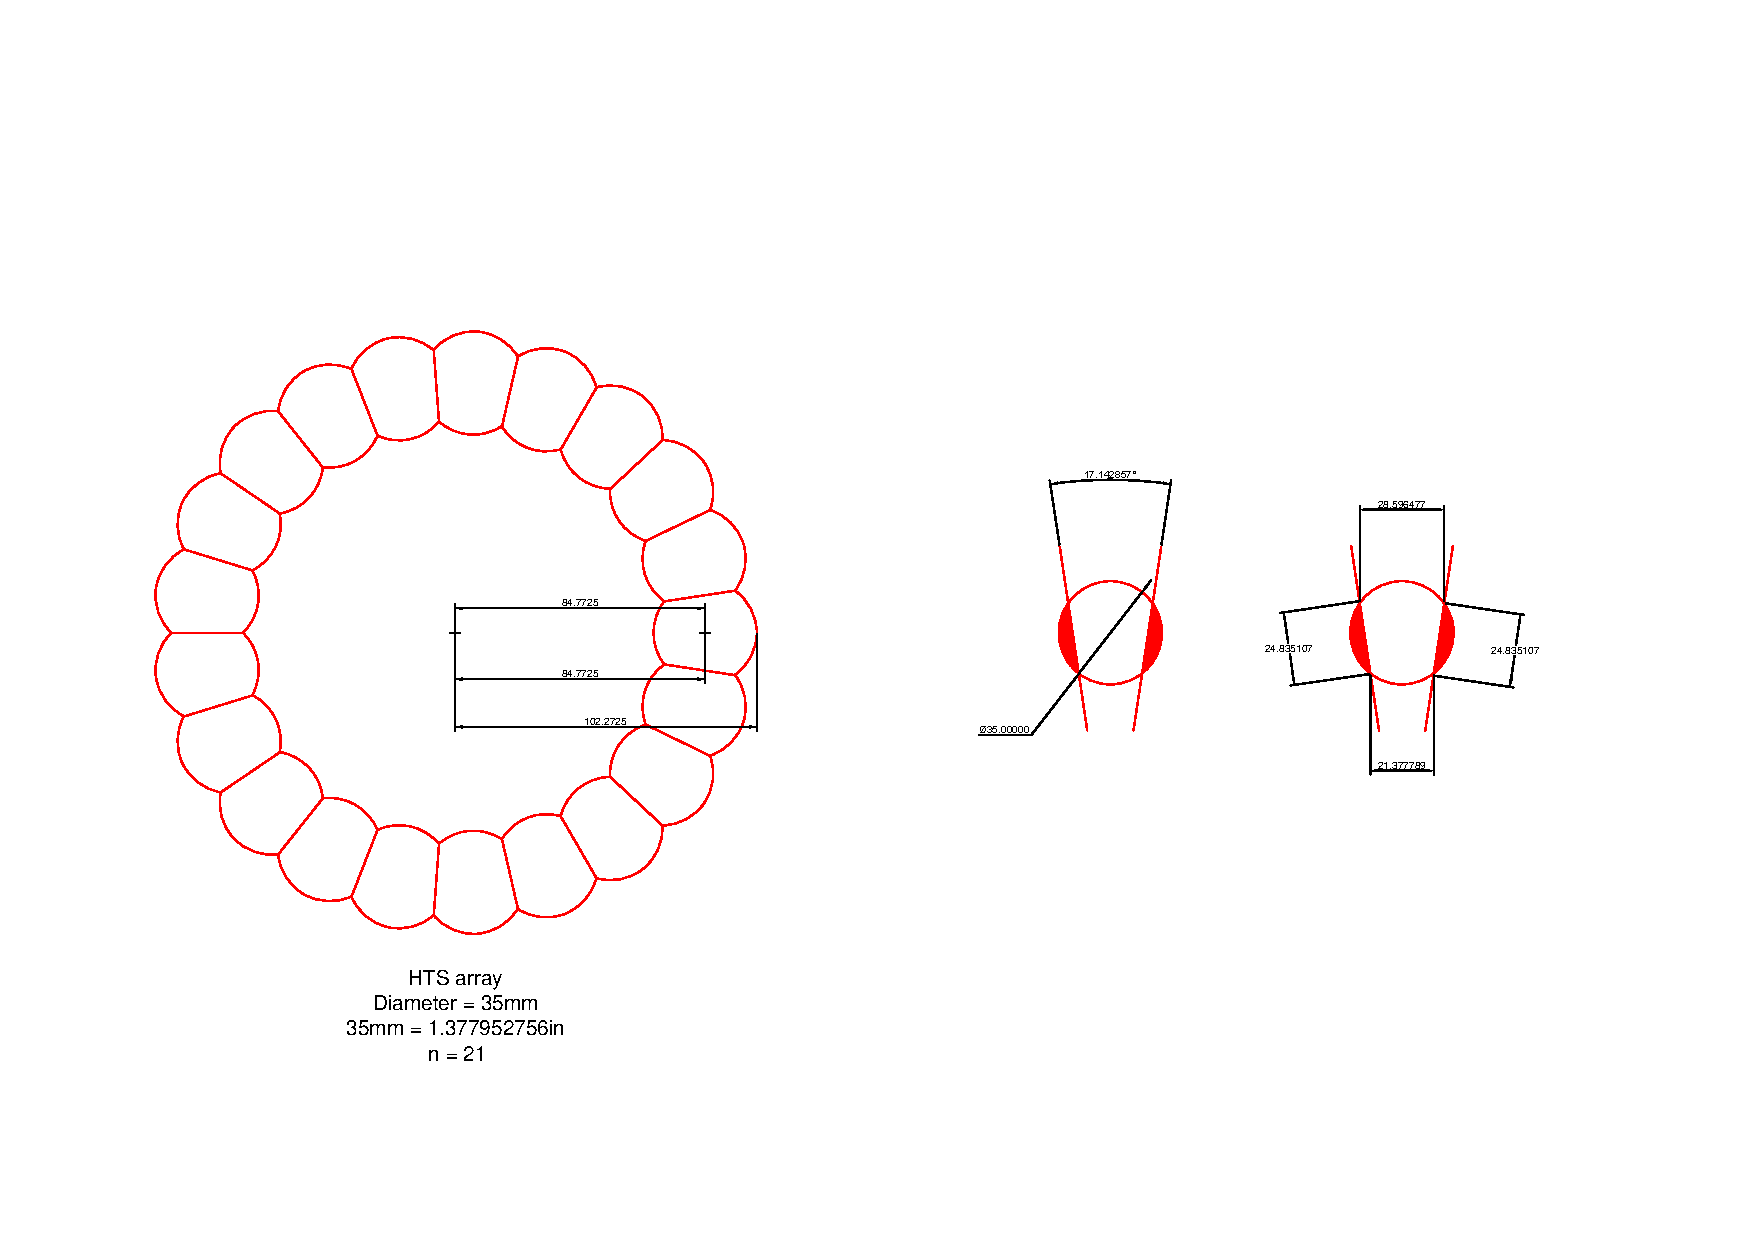
\includegraphics[scale=0.65, clip=true, trim=2cm 3.75cm 15cm 5cm]{HTS_Array.pdf}
\caption{HTS wedge shaped samples cut from Diameter=35mm cylinders ordered from and shaped by Can-superconductors.}
\label{fig_HTS_Samples}
\end{figure}

\begin{figure}[htbp]
\centering
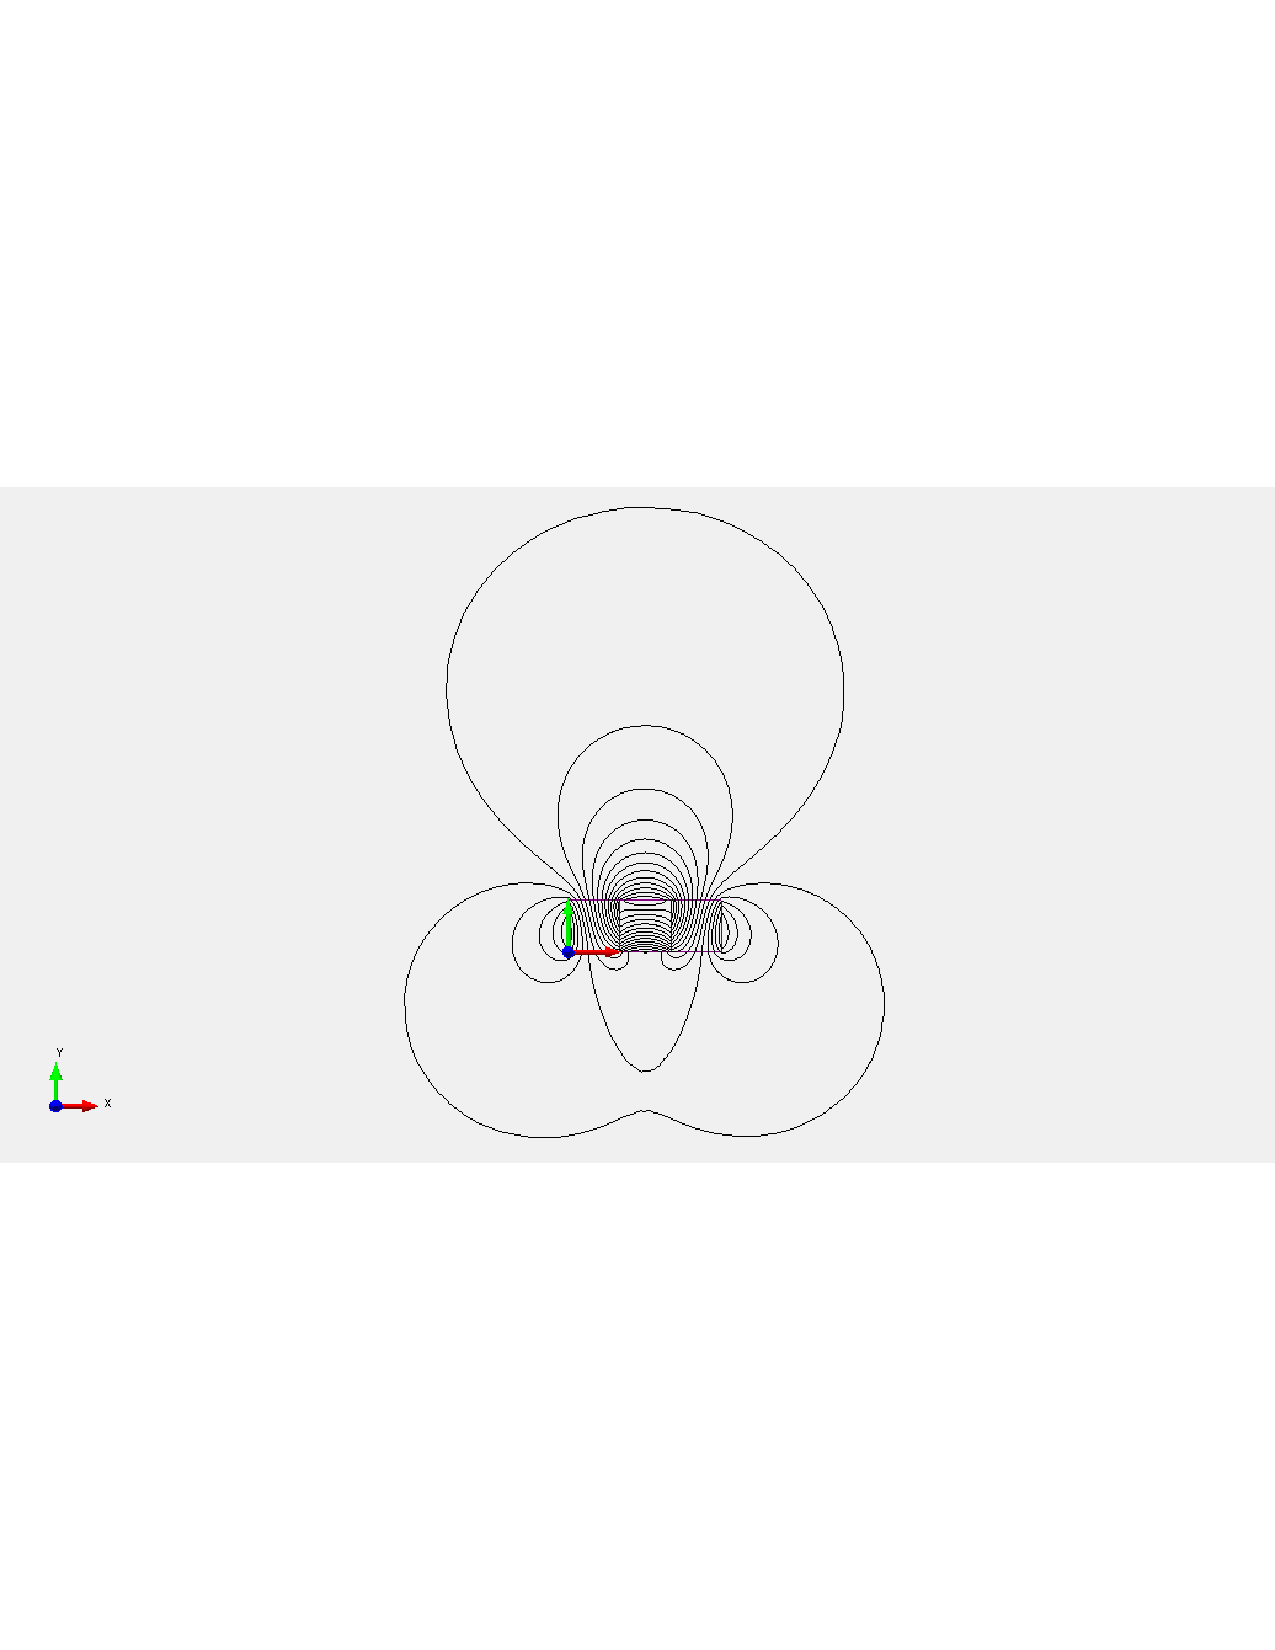
\includegraphics[scale=0.3, clip=true, trim=0cm 5cm 0cm 5cm]{3MagsFluxProfile_12.pdf}
\caption{Flux profile of profile 12 in the orientation $\uparrow \leftarrow \downarrow$.}
\label{fig_fluxprofile_12}
\end{figure}

\begin{figure}[htbp]
\centering
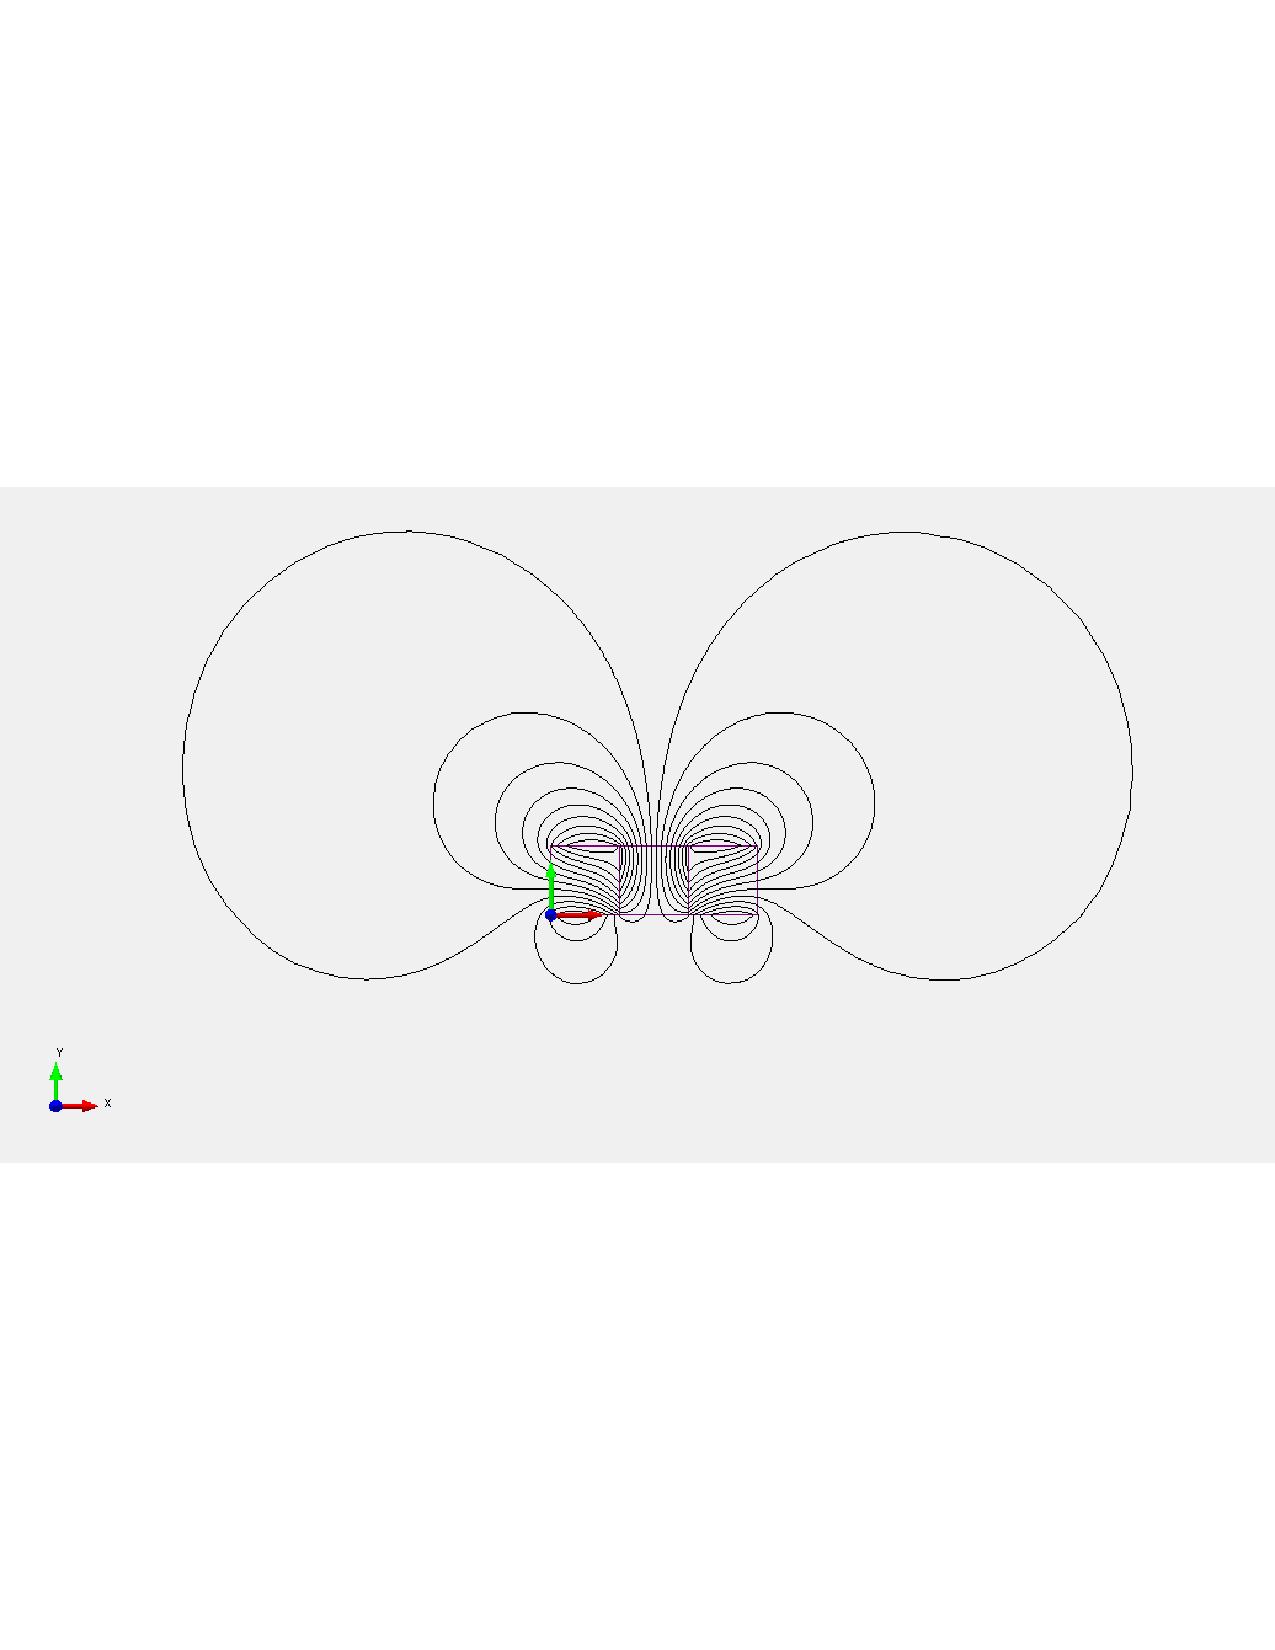
\includegraphics[scale=0.3, clip=true, trim=0cm 5cm 0cm 5cm]{3MagsFluxProfile_19.pdf}
\caption{Flux profile of array 19 in the orientation $\rightarrow \uparrow \leftarrow$.}
\label{fig_fluxprofile_19}
\end{figure}

\begin{figure}[htbp]
\centering
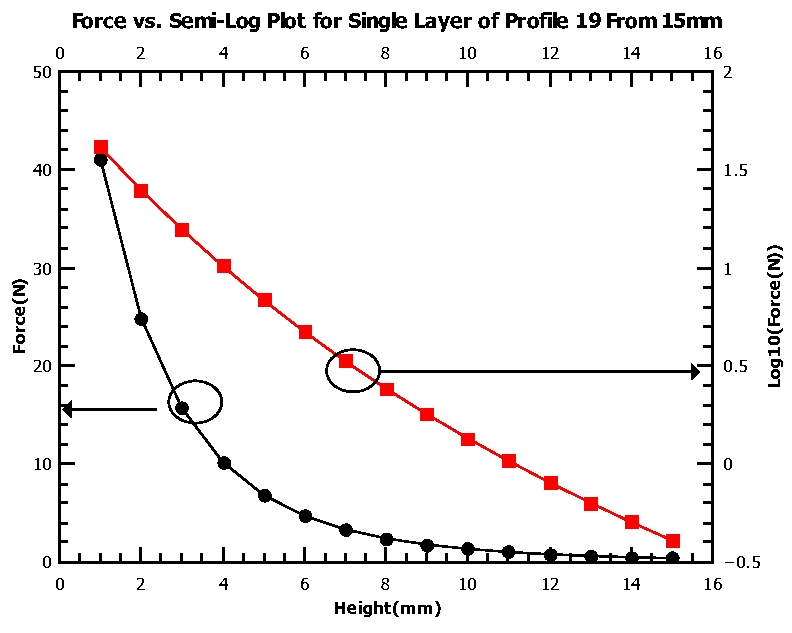
\includegraphics[width=3in]{ForceSemiPro19.pdf}
\caption{Semi-Log plot for FEA using profile 19 in a single layer.  The data was truncated at a maximum of 15 mm for the range of interest.}
\label{fig_force19_one}
\end{figure}

\begin{figure}[htbp]
\centering
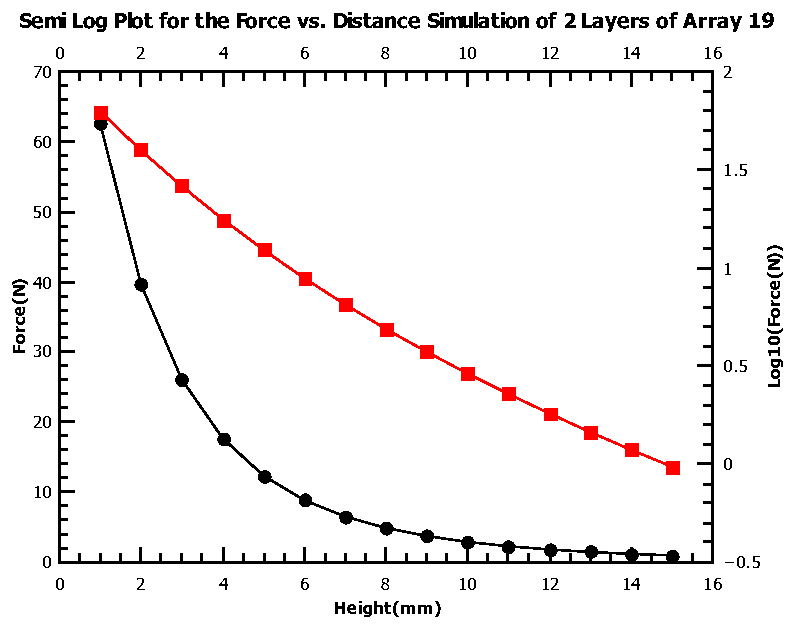
\includegraphics[width=3in]{SemiLogArr192LayersAt15mm.pdf}
\caption{Semi Log plot of the simulation force against two layers of profile 19 truncated at a maximum height of 15mm.}
\label{fig_force19_two}
\end{figure}

\begin{figure}[htbp]
\centering
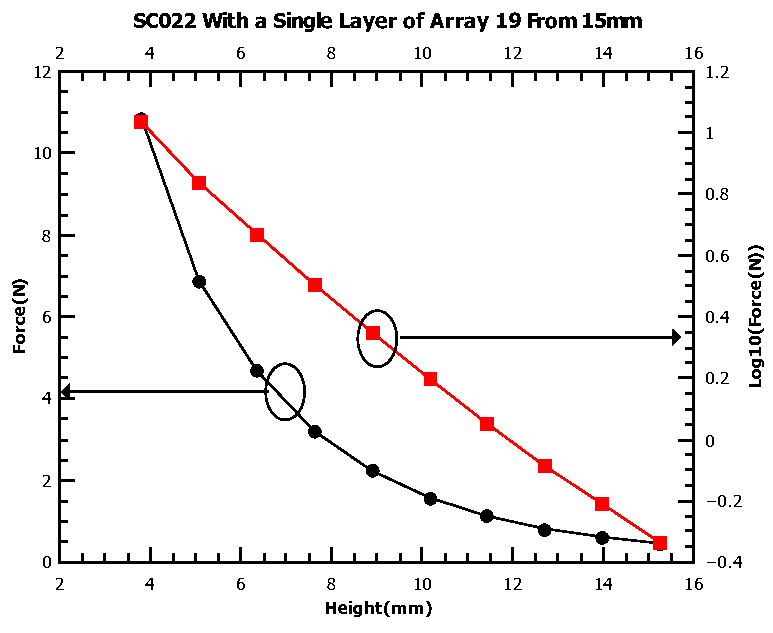
\includegraphics[width=3in]{SC022singleWith19.pdf}
\caption{Semi-Log plot of experiment using SC022 against a single layer of magnets using profile 19.  The data was truncated at a maximum of 15 mm for the range of interest.}
\label{fig_force22_one}
\end{figure}

\begin{figure}[htbp]
\centering
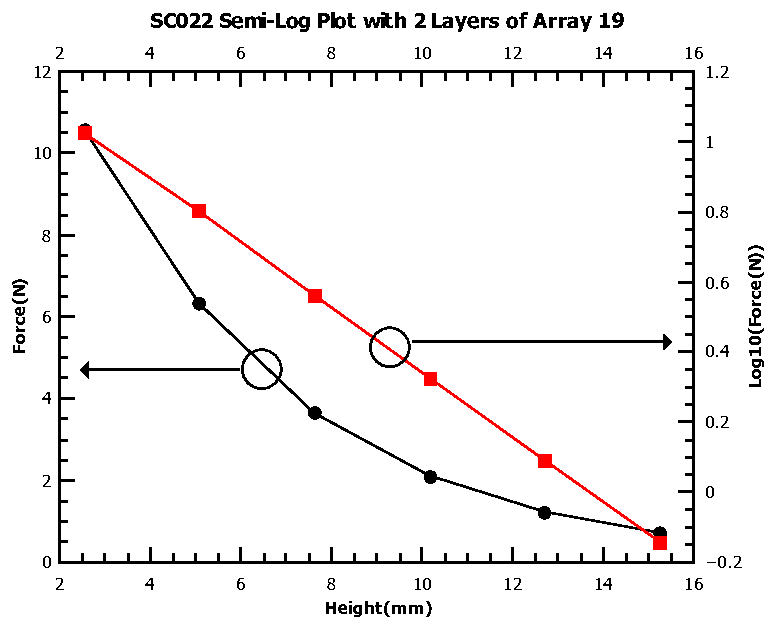
\includegraphics[width=3in]{SC022DoubleWith19.pdf}
\caption{Semi Log plot of the experimental force using SC022 and two layers of array 19 truncated at a maximum height of 15mm.}
\label{fig_force22_two}
\end{figure}

\begin{figure}[htbp]
\centering
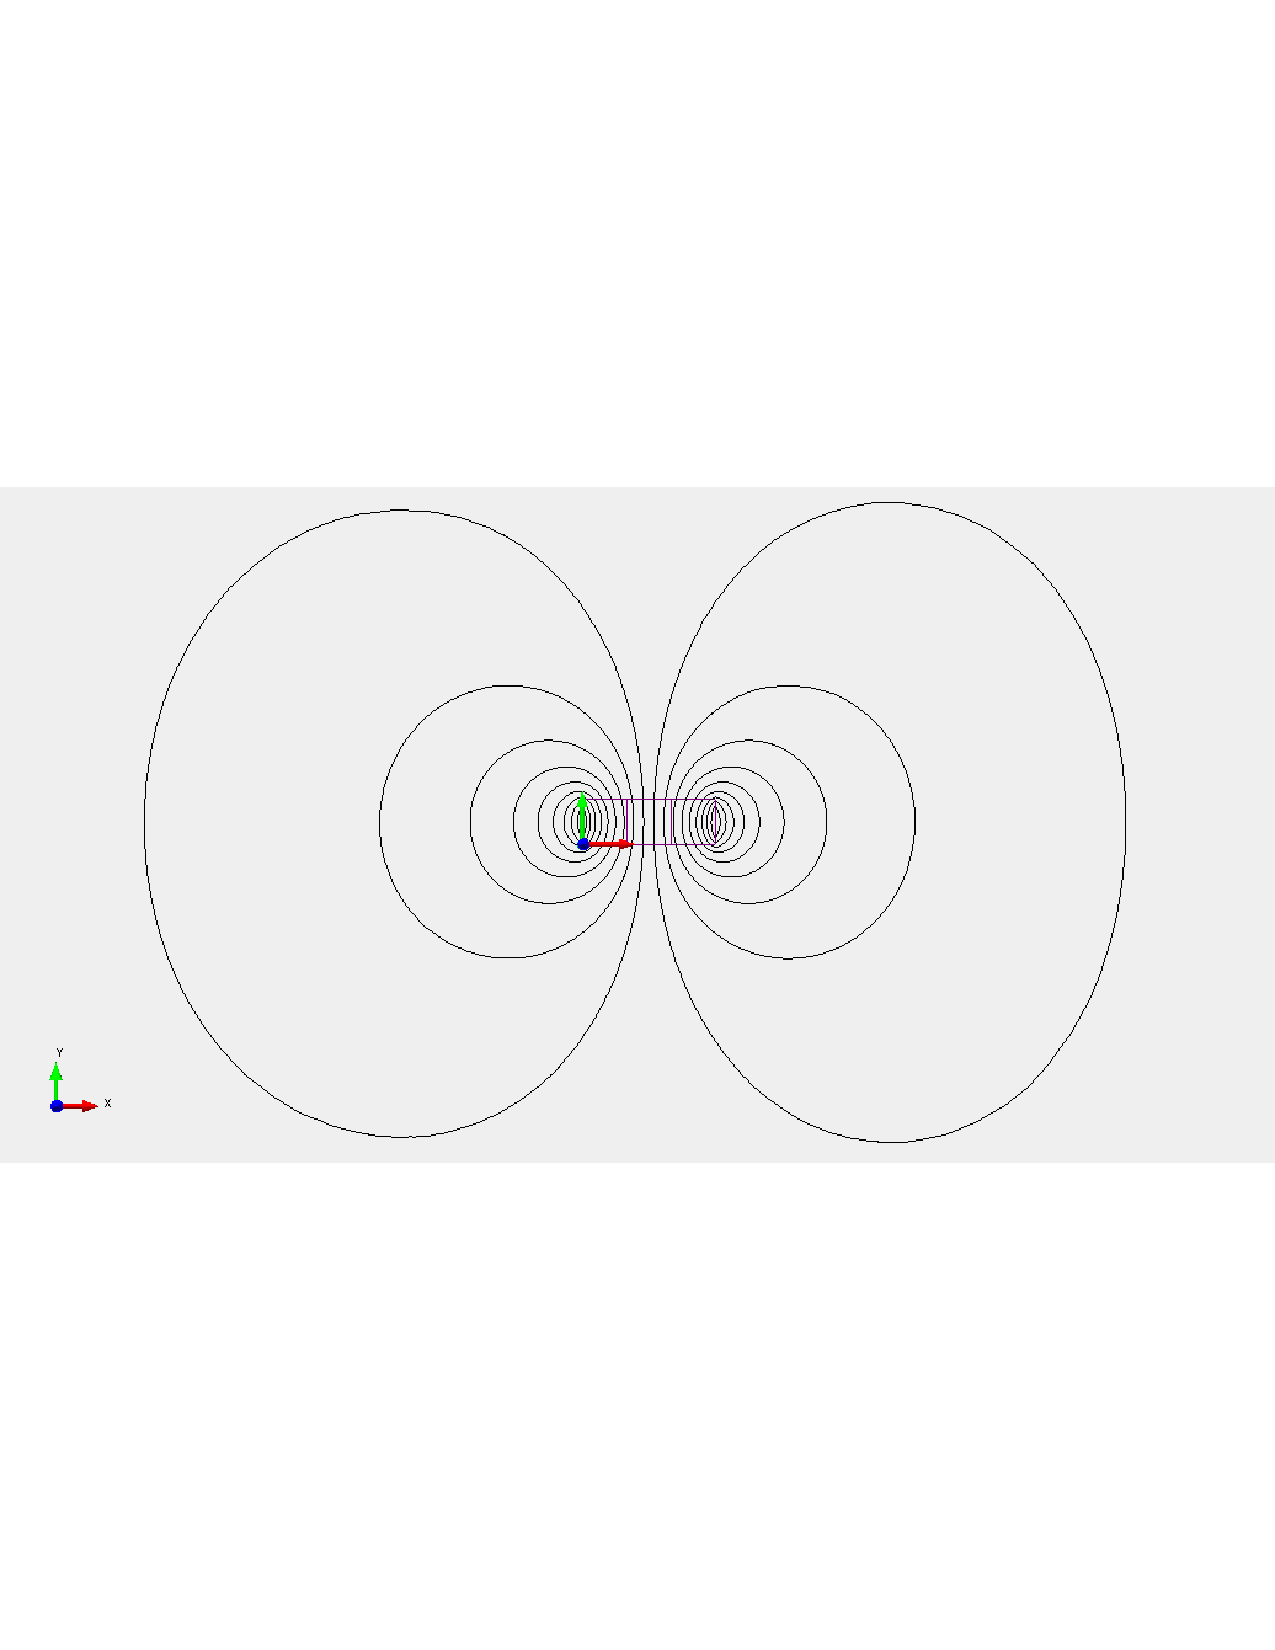
\includegraphics[scale=0.3, clip=true, trim=0cm 5cm 0cm 5cm\textwidth]{figures/FluxProfile1SingleLayer.pdf}
\caption{Flux profile of profile 1 in the orientation $\uparrow \uparrow \uparrow$.}
\label{fig_fluxprofile_1}
\end{figure}

\begin{figure}[htbp]
\centering
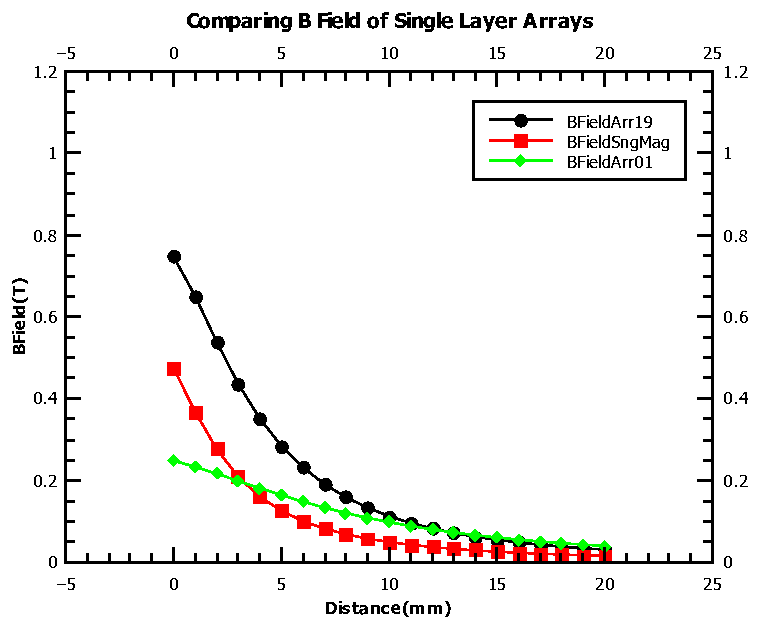
\includegraphics[width=3in]{BFieldSnLs.pdf}
\caption{Using FEA simulation data we compare the magnetic field between a single cube magnet, a single layer of profile 19 (three magnets in the orientation $\rightarrow\uparrow\leftarrow$) and a single layer of profile 1 (three magnets in the orientation $\uparrow\uparrow\uparrow$).}
\label{fig_BFieldSnLs}
\end{figure}

\begin{figure}[htbp]
\centering
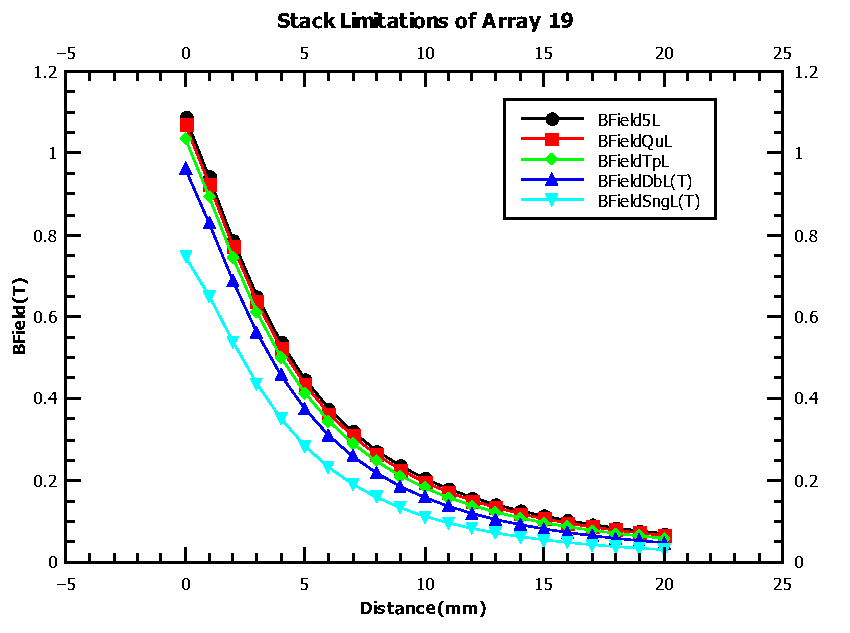
\includegraphics[width=3in]{StckLimArr19.pdf}
\caption{The simulation data shows a limitation in the increase of the B-field as a function of height from adding additional layers of profile 19.  The increase  drops off quickly after 3 layers.}
\label{fig_StckLimArr19}
\end{figure}

\begin{figure}[htbp]
\centering
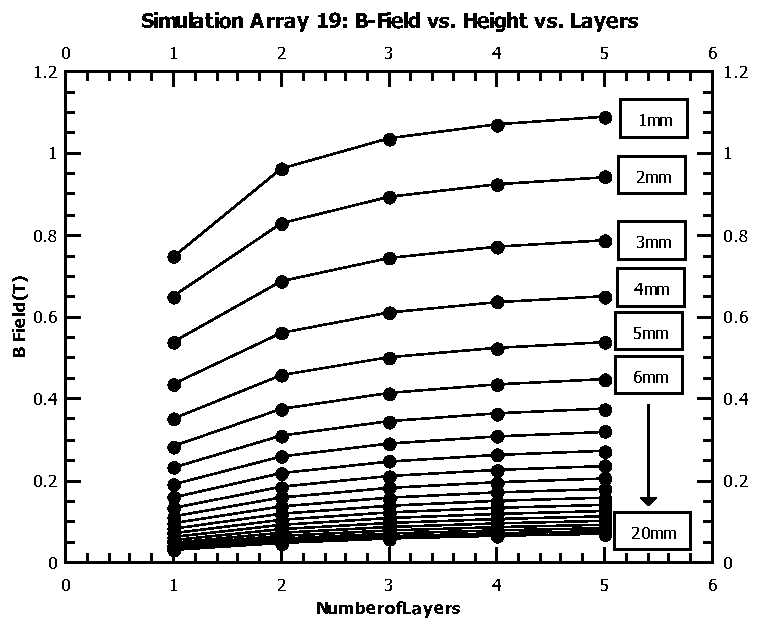
\includegraphics[width=3in]{BFieldVsLayerArr19.pdf}
\caption{Simulation data of the B-field from profile 19 as a function of the number of layers.  Each line represents an increase in the distance between superconductor and magnet array.}
\label{fig_BFieldVsLayerArr19}
\end{figure}

\begin{figure}[htbp]
\centering
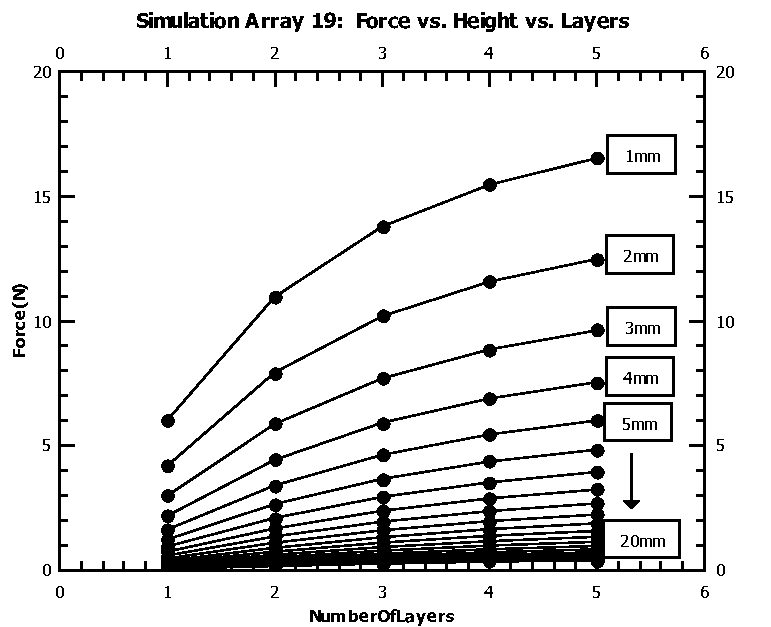
\includegraphics[width=3in]{FVsHVsLArr19.pdf}
\caption{Simulation data of the Force from profile 19 as a function of the number of layers.  Each line represents an increase in the distance between superconductor and magnet array.}
\label{fig_ForceVsLayerArr19}
\end{figure}

\begin{figure}[htbp]
\centering
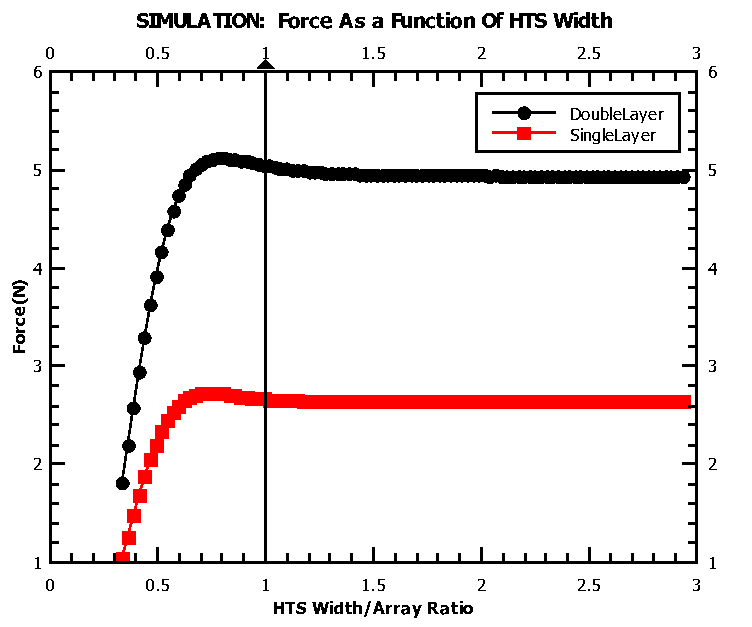
\includegraphics[width=3.3in]{ForceFncWidthArrOneAndTwoLyrs.pdf}
\caption{Simulation results of the force versus varying width of the HTS against profile 19.  The HTS maintained a height of 6.35mm but the width was slowly increased. }
\label{fig_ForceWidthArr19}
\end{figure}

\begin{figure}[htbp]
\centering
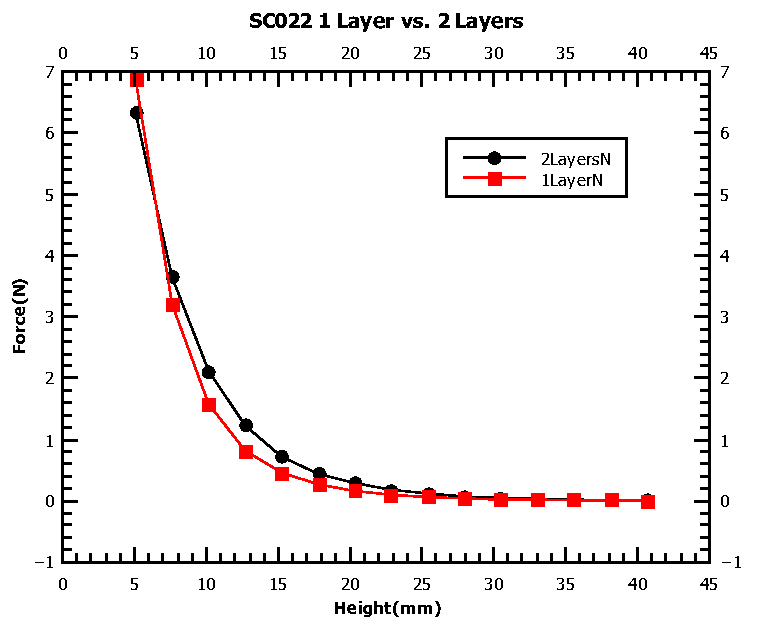
\includegraphics[width=3in]{figures/SC0221LayerVs2Layers.pdf}
\caption{Experimental result of the force on a HTS with 1 and 2 layers of profile 19. There is no significant increase at 5-7mm.}
\label{fig_1layervs2}
\end{figure}

\begin{figure}[htbp]
\centering
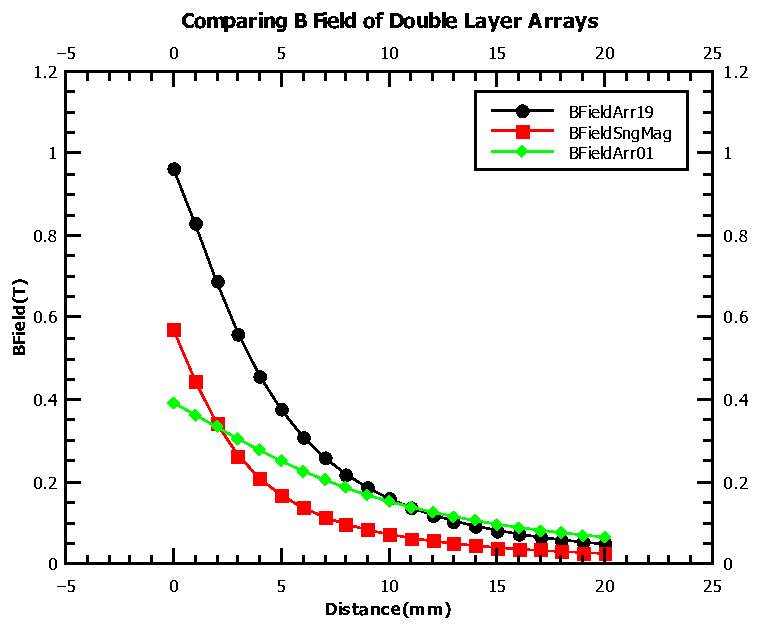
\includegraphics[width=3in]{BFieldDbLs.pdf}
\caption{Using FEA simulation data we compare the magnetic field between two stacked cube magnets, a double layer of profile 19 (three magnets in the orientation $\rightarrow\uparrow\leftarrow$) and a double layer of profile 1 (three magnets in the orientation $\uparrow\uparrow\uparrow$).}
\label{fig_BFiledDbLs}
\end{figure}